\chapter{附录}
\label{sec.appendix}

\section{校园地图}
\begin{figure}[H]
    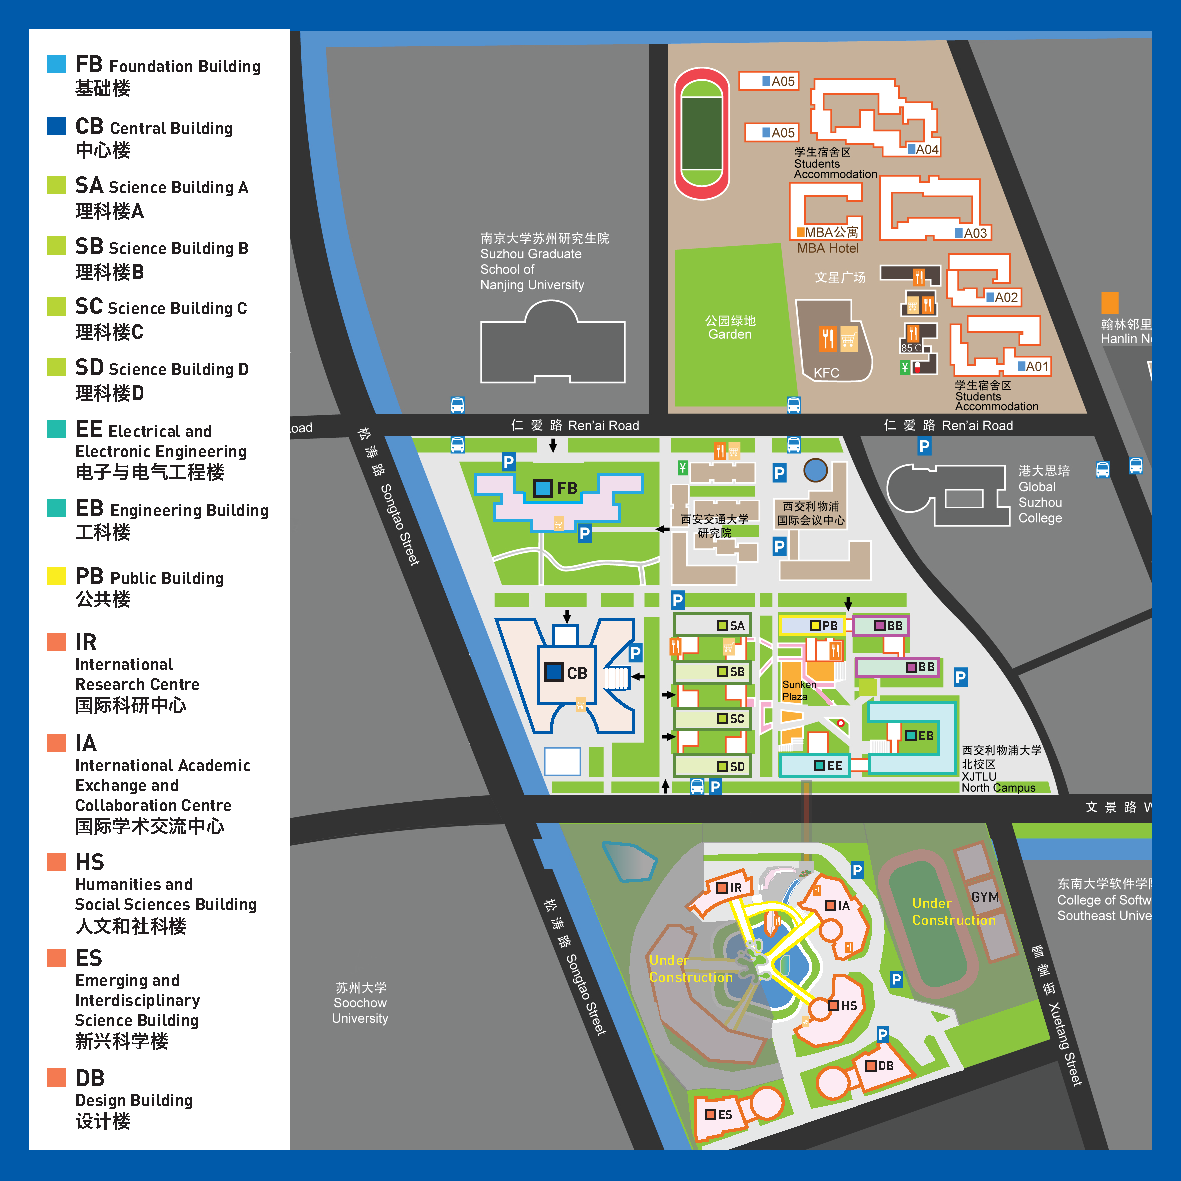
\includegraphics[width=\columnwidth]{author-folder/Kai.Wu/XJTLU-campus-map.pdf}
\end{figure}

\clearpage
% \section{校历:哪天放假}
% 独立的校历文件可在本项目的GitHub里(\href{https://github.com/kaiwu-astro/xp_pgrs_unofficial_guide/raw/main/author-folder/Kai.Wu/Academic_Calendar-202223.pdf}{链接})找到。
% \begin{figure}[H]
%     \includegraphics[width=0.9\columnwidth]{author-folder/Kai.Wu/Academic_Calendar-202223.pdf}
% \end{figure}

\section{学校电话}

\begin{table}[H]
    \begin{tabular}{p{60mm}cc}
        \hline
        部门 & 电话 & 邮箱 \\ \hline
        Academic Services Office \newline 学术服务 & 8188 4754 & aso@xjtlu.edu.cn \\ \hline
        Alumni Service \newline 校友服务           & 8816 1869 & alumni@xjtlu.edu.cn \\ \hline
        Campus Management Office\newline 校园管理办公室 & 8816 1071 & cmo@xjtlu.edu.cn \\ \hline
        Career Service \newline 就业服务           & 8188 8308 & careers@xjtlu.edu.cn \\ \hline
        IT Service Centre \newline IT服务中心      & 8816 1250 & it@xjtlu.edu.cn \\ \hline
        Library \newline 图书馆                    & 8816 1290 & askalibrarian@xjtlu.edu.cn \\ \hline
        Media Service \newline 新闻线索与媒体服务    & 8816 1351/1032 & news@xjtlu.edu.cn \\ \hline
        Postgraduate Recruitment \newline 研究生招生 & 8816 1889/7111 & pgenquiries@xjtlu.edu.cn \\ \hline
        President's Office \newline 校长办公室     & 8816 1004 & president.office@xjtlu.edu.cn \\ \hline
        Registry \newline 教务办公室               & 8816 1230 & registry@xjtlu.edu.cn \\ \hline
        Research Management Office \newline 科研管理办公室 & 8816 1139 &  \\ \hline
        Student Onestop Centre \newline 学生一站式 & 8816 1854 & onestop@xjtlu.edu.cn \\ \hline
        XJTLU Global (Support) \newline 西浦国际 & 8897 3094/3093 & global@xjtlu.edu.cn \\ \hline
    \end{tabular}
\end{table}
\clearpage

\section{加入我们:评论机制及委员会化运作动议}
\textbf{摘要:} \textit{本攻略已经覆盖了西浦博士生从入学到毕业的多类重要信息和经验,已经事实上成为唯一的从西浦博士生视角出发的成体系攻略。但是,攻略也有可持续性的问题,为此我们提出了包括组织同行评议、组织 workshop、扩充供稿渠道、寻求运营经费、设置运营委员会等在内的调整动议。我们热切欢迎任何愿意参与的同学及一切可能的帮助。}

可喜可贺,历时两年半,我们的《西浦博士生非官方攻略》已经有了六个正文章节!除原有的\href{https://github.com/xp-pgrs-unofficial-guide/xp_pgrs_unofficial_guide/releases}{中文版}之外,我们也在推进\href{https://github.com/xp-pgrs-unofficial-guide/xp_pgrs_unofficial_guide_EN/releases}{英文版}的翻译工作。
感谢各位编辑及撰稿同学的努力,这本攻略的内容已经覆盖了西浦博士生从入学到毕业的多类重要信息和经验。

不过,我们目前的内容管理完全依赖同学们个人的为爱发电。选题、撰稿均依赖供稿同学的个人经验;在一些时候,由编辑同学撰稿的内容无人审核。考虑到整个攻略的体量,我目前能做的也仅是依据个人经验增加一些章节内容,或对其他同学供稿的大致内容进行审核并将其加入到已经略显臃肿的目录中。这对我们的攻略来说无疑是一个灾难:无人审核或经过审核但缺乏可靠性(后者更可怕)的内容无疑会降低攻略的价值。

所幸,攻略本身具有一些价值让我们可以做一些事情尝试改变这个局面。以我所知,这仍然是目前唯一的一份从西浦博士生视角出发的多角度成体系攻略:其涵盖的内容远超任一学校部门的责任范围,使得校官方文件很难在内容广度上与之相比;攻略内容完全由西浦在读或已毕业博士生同学撰写、编辑,以同学们更好理解的视角出发制作;攻略内容积累超两年,由多位同学撰稿、编辑,其体量及规整度也远超任一其他经验贴、攻略。

\vspace{5mm}

为此,我计划对攻略的运作方式做出一些调整,以更好的发挥攻略的价值:
\begin{itemize}
    \item 设置评论机制。来自于除了撰稿人、编辑之外的其他同学的经验和知识对于攻略的内容质量非常重要,我计划在攻略的制作阶段增加评论环节,供大家对已有及新增内容进行评论。这可以帮助维护攻略内容的质量,也能发现尚未覆盖的内容作为新内容的线索。为此,我计划在已有的开源平台之外,增加评论机制,供同学们对攻略内容进行评论,希望能提供更方便使用的方式引入同学们的建议。编辑将根据评论内容调整攻略编制,或与实际撰稿人联系对内容进行调整。提供被采纳意见的同学将同样被列入攻略的贡献者名单。
    \item 组织 workshop 活动。攻略本身覆盖了大量议题,而受限于篇幅及需要投入的时间,我们几乎不可能在短时间内形成一份包含了每个议题下所有观点的版本。为此,我们计划组织针对不同议题的 workshop,以帮助增进了解、交流观点、补充攻略,同时我们也希望此类活动可以成为学习生活中的一份调剂。
    \item 扩充约稿渠道。以往,攻略内容来自于撰稿同学的自发投稿,或由编辑邀请熟识同学撰稿。在当前攻略的体量下,这一模式要求编辑同学能在学习之余抽出大量闲暇时光贡献于攻略,现已难以为继。为此,我计划利用同行评议和 workshop 活动作为额外的约稿来源。对于在同行评议中发现的尚未覆盖的内容,将定期向全体博士在校及已毕业同学发布,征集内容;同时根据 workshop 中的独特观点,邀请同学撰稿。
    \item 寻求运营经费。显然,无论是组织同行评议、workshop,还是未来的其他事情,我们都需要或多或少的在赋予它们意义之外支付费用,这无疑对攻略的可持续运营有更多的正向作用。为此,我计划接下来尝试包括寻求赞助、合作等方式寻求运营经费。
    \item 扩充编辑团队。考虑到以上所有的潜在工作内容,以及在推进的英文版,我们会需要额外的编辑同学加入。目前空缺至少 1 位中文版编辑和 1 位英文版编辑。英文版目前已经完成了利用大模型的中文到英文的翻译,但后续内容校对的组织、面向国际生同学的独特内容的编辑仍然充满挑战。
    \item 设置运营委员会。无论是组织攻略编辑、各类活动,还是寻求运营经费,这都不是只靠个人的闲暇时光就能完成的。为此,我计划设置攻略的运营委员会作为攻略运作的主体,完全负责攻略的全部工作。与目前仅依赖编辑完成所有组织管理的方式不同,委员会依赖各位委员依个人不同能力领导各类事物。委员会不设固定席位、无名额上限,但原则上仅接纳对攻略运营有重大影响力的个人或组织代表,并限制非博士生在校生、校友的委员数量。
    
\end{itemize}

\vspace{5mm}

各位,如果你对参与以上的任一事情感兴趣,或有其他有助于改进攻略运作方式的想法,欢迎直接联系我 (\email{shiyao.zhang14@student.xjtlu.edu.cn})。我们热切欢迎任何愿意参与的同学及一切可能的帮助!目前这仍然是一份动议,但我计划在今年推进对攻略运作方式的调整并取得一些改变。

\begin{flushright}
    编辑 \Shiyao\\
    2025年2月11日
\end{flushright}